% begin module arcsin-def
\begin{frame}
\frametitle{Inverse Trigonometric Functions}
\ \only<handout:0| -1>{%
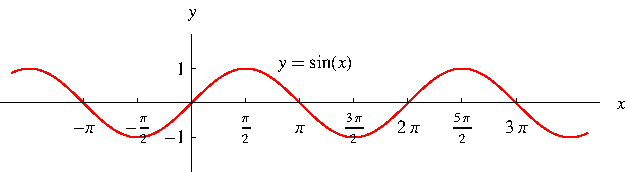
\includegraphics[width=12cm]{inverse-trig/pictures/07-06-arcsina.pdf}%
}%
\only<handout:0| 2>{%
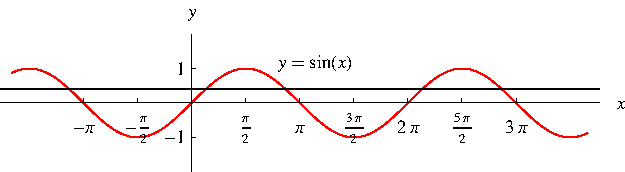
\includegraphics[width=12cm]{inverse-trig/pictures/07-06-arcsinb.pdf}%
}%
\only<3>{%
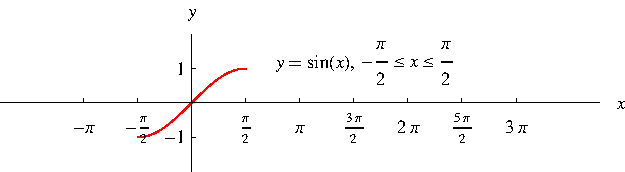
\includegraphics[width=12cm]{inverse-trig/pictures/07-06-arcsinc.pdf}%
}%
\only<handout:0| 4->{%
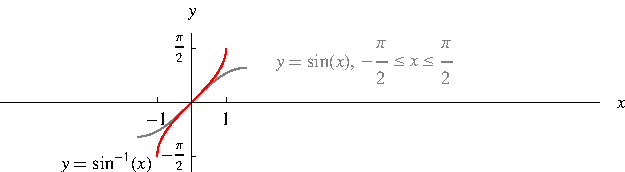
\includegraphics[width=12cm]{inverse-trig/pictures/07-06-arcsind.pdf}%
}%
\begin{columns}[c]
\column{.65\textwidth}
\begin{itemize}
\item<2->  $\sin x$ isn't one-to-one.
\item<3->  It is if we restrict the domain to $[-\pi /2, \pi /2]$.
\item<4->  Then it has an inverse function.
\item<4->  We call it $\sin^{-1}$ or $\arcsin$.
\item<6->  $\sin^{-1} (x) = y \Leftrightarrow \sin y = x$ and $-\pi /2 \leq y \leq \pi /2$.
\end{itemize}
\column{.35\textwidth}
\uncover<5->{%
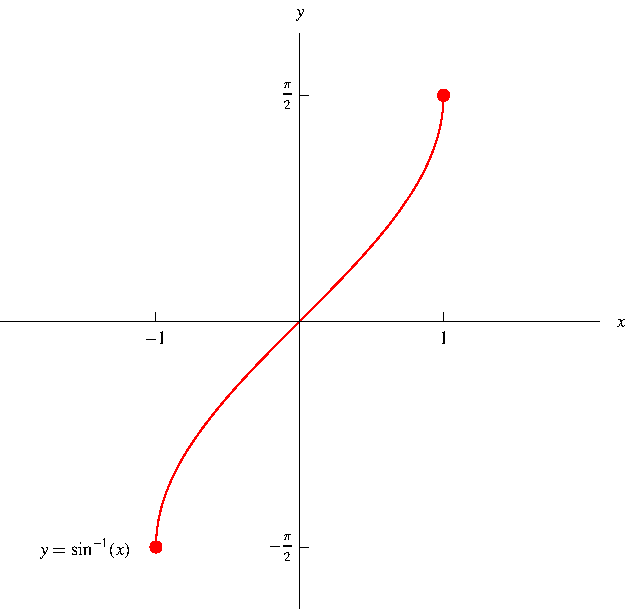
\includegraphics[height=4cm]{inverse-trig/pictures/07-06-arcsine.pdf}%
}%
\end{columns}
\end{frame}
% end module arcsin-def
